\documentclass{../source/Experiment}
\usepackage{multirow}
\major{信息工程}
\name{姚桂涛}
\title{一阶RC电路的瞬态响应过程}
\stuid{3190105597}
\college{信息与电子工程学院}
\date{\today}
\lab{东4-216}
\course{电子电路设计实验}
\instructor{李锡华、施红军、叶险峰}
\grades{}
\expname{一阶RC电路的瞬态响应过程}
\exptype{研究实验}
\partner{杜秉哲}

\begin{document}
    \makecover
    \makeheader

    \section{实验目的}
        \begin{enumerate}
            \item 熟悉一阶RC 电路的零状态响应、零输入响应过程。
            \item 研究一阶RC 电路在零输入、阶跃激励情况下,响应的基本规律和特点。
            \item 学习用示波器观察分析RC 电路的响应。
            \item 从响应曲线中求RC 电路的时间常数。
        \end{enumerate}
    \section{实验任务和要求}
        \begin{enumerate}
            \item 按电路图连接好电路。
            \item 用示波器观察RC电路的零输入响应、零状态响应,描绘响应曲线,求出电路的时间常数。
            \item 更换电路中电阻、电容的大小(即改变时间常数),重新测量电路的各种响应,分别求出每次测量的时间常数。
            \item 理论计算(仿真)电路的时间常数,并与实验测量值比较。
        \end{enumerate}
    \section{实验方案设计与实验参数计算}
        \subsection{完整实验电路}
            % \newpage
            \begin{figure}[htbp]
                \centering
                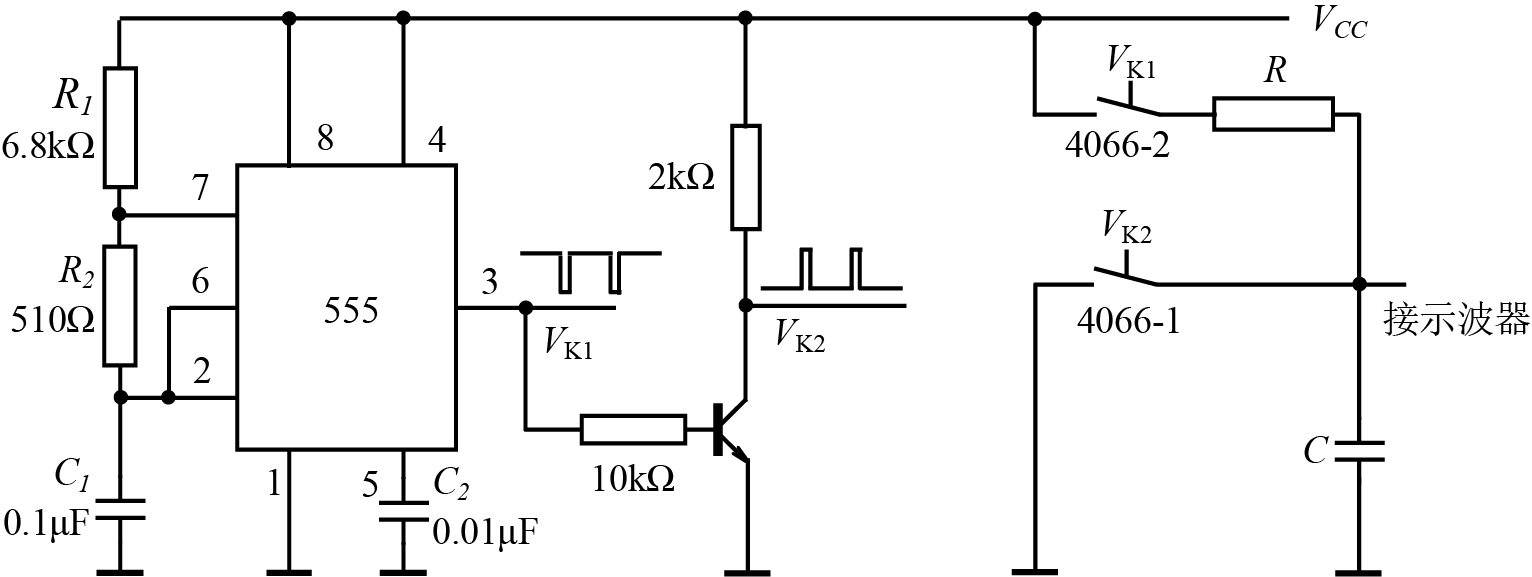
\includegraphics[scale = 0.8]{rc1}
                \caption{完整实验电路}
            \end{figure}
        \subsection{实验方案总体设计}
            \begin{enumerate}
                \item 按电路图连接好实验电路
                \item 示波器观察$RC$零输入相应电路,描绘响应曲线,求出电路的时间常数。并改变电容,再次实验。
                \item 示波器观察$RC$零状态相应电路,描绘响应曲线,求出电路的时间常数。并改变电阻,再次实验。
                \item 理论计算出各个电路的时间常数值与实验测量值比较。
            \end{enumerate}
    \section{主要仪器设备}
            示波器,实验电路板。
    \section{实验步骤、实验调试过程、实验数据记录}
        \subsection{实验步骤以及实验调试过程}
            \begin{enumerate}
                \item 按电路图连接好实验电路。
                \item 示波器观察$RC$零输入相应电路,描绘响应曲线,根据如图2公式,测量出时间常数,记入表中。
                \item 更换电路中的电容,重复(2)实验。
                \item 示波器观察$RC$零状态相应电路,描绘响应曲线,根据如图3公式,测量出时间常数,记入表中。
                \item 更换电路中的电阻,重复(4)实验。
                \item 理论计算出每个实验的时间常数记入表中。
            \end{enumerate}
            % \newpage
            \begin{figure}[htbp]          
                \begin{minipage}[t]{0.5\textwidth}
                    \centering
                    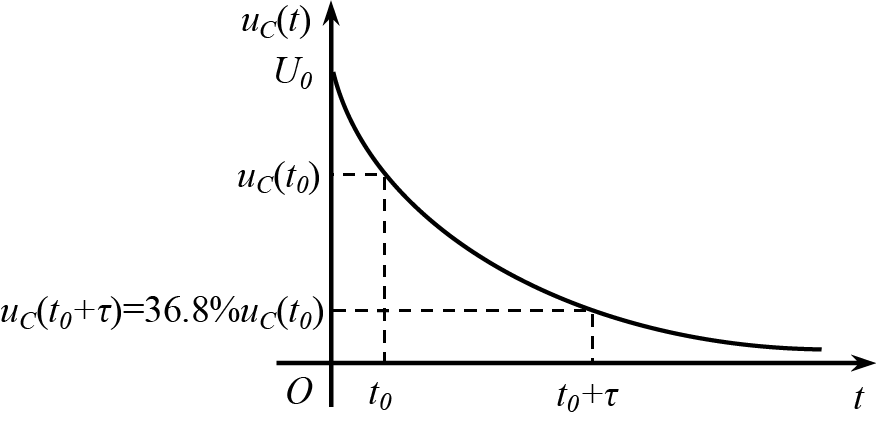
\includegraphics[scale=0.8]{pic/rc2.png}
                    \caption{零输入响应\label{fig:1}}
                \end{minipage}
                \qquad
                \begin{minipage}[t]{0.5\textwidth}
                    \centering
                    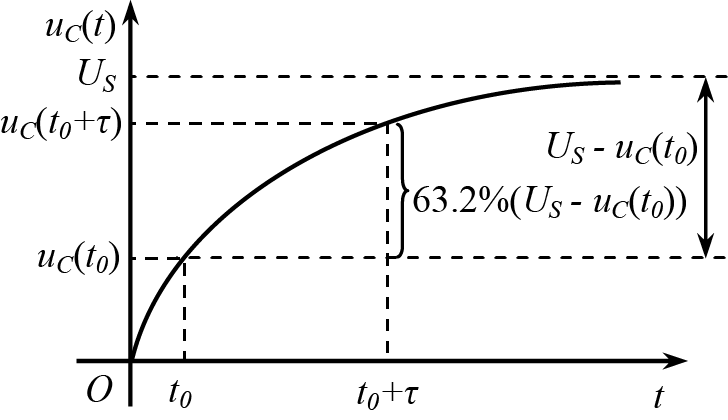
\includegraphics[scale=0.8]{rc3}
                    \caption{零状态响应\label{fig:2}}
                \end{minipage}
            \end{figure}
        \subsection{实验数据记录}
            \newpage
            \begin{table}[htbp]
                \centering
                \caption{$RC$时间常数的测量}
                \begin{tabular}{c|c|c|c|c|c}
                    \hline
                    Num & $R$   & $C$    & $\tau$ (测量值)   & $\tau '$ (计算值) &                        \\ \hline
                    1 & $4.3k\Omega$ & $0.22\mu F$ & $9.4\times 10^{-4}s$ & $9.46\times 10^{-4}s$ & \multirow{2}{*}{零输入响应} \\ \cline{1-4}
                    2 & $4.3k\Omega$ & $0.01\mu F$ & $4.2\times 10^{-5}s$ & $4.3\times 10^{-5}s$ &                        \\ \hline
                    3 & $9.1k\Omega$ & $0.1\mu F$ & $9.2\times 10^{-4}s$ & $9.1\times 10^{-4}s$ & \multirow{2}{*}{零状态响应} \\ \cline{1-4}
                    4 & $750\Omega$ & $0.1\mu F$ & $8.4\times 10^{-5}s$ & $7.2\times 10^{-5}s$ &                        \\ \hline
                \end{tabular}
            \end{table}
    \section{实验结果和分析处理}
        \subsection{数据分析}
        \begin{table}[htbp]
            \centering
            \caption{$RC$时间常数的测量}
            \begin{tabular}{c|c|c|c|c|c}
                    \hline
                    Num & $R$   & $C$    & $\tau$ (测量值)   & $\tau '$ (计算值) &                        \\ \hline
                    1 & $4.3k\Omega$ & $0.22\mu F$ & $9.4\times 10^{-4}s$ & $9.46\times 10^{-4}s$ & \multirow{2}{*}{零输入响应} \\ \cline{1-4}
                    2 & $4.3k\Omega$ & $0.01\mu F$ & $4.2\times 10^{-5}s$ & $4.3\times 10^{-5}s$ &                        \\ \hline
                    3 & $9.1k\Omega$ & $0.1\mu F$ & $9.2\times 10^{-4}s$ & $9.1\times 10^{-4}s$ & \multirow{2}{*}{零状态响应} \\ \cline{1-4}
                    4 & $750\Omega$ & $0.1\mu F$ & $8.4\times 10^{-5}s$ & $7.2\times 10^{-5}s$ &                        \\ \hline
            \end{tabular}
        \end{table}
        \par 
        曲线描绘\\
        % \newpage
        \begin{figure}[htbp]          
                \begin{minipage}[t]{0.5\textwidth}
                    \centering
                    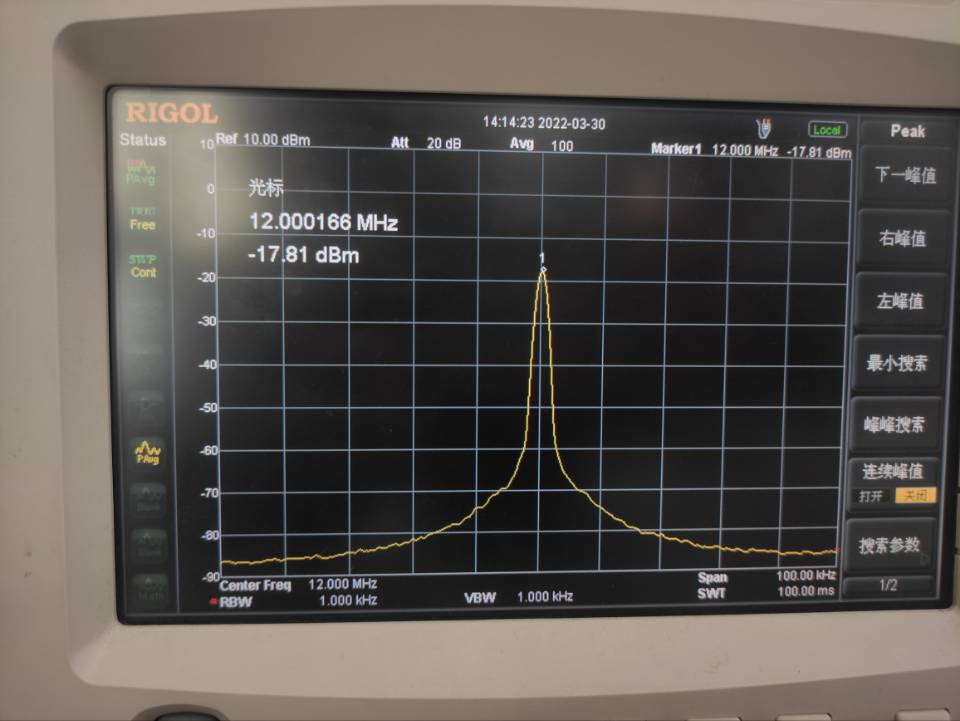
\includegraphics[scale=0.8]{1}
                    \caption{零输入响应1\label{fig:1}}
                \end{minipage}
                \quad
                \begin{minipage}[t]{0.5\textwidth}
                    \centering
                    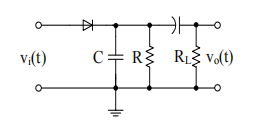
\includegraphics[scale=0.8]{2}
                    \caption{零输入响应2\label{fig:2}}
                \end{minipage}
                \quad 
                \begin{minipage}[t]{0.5\textwidth}
                    \centering
                    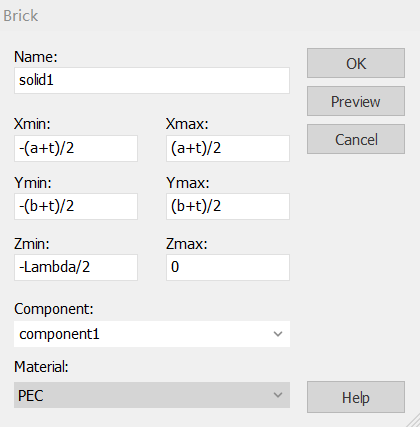
\includegraphics[scale=0.8]{3}
                    \caption{零状态响应1\label{fig:2}}
                \end{minipage}
                \quad 
                \begin{minipage}[t]{0.5\textwidth}
                    \centering
                    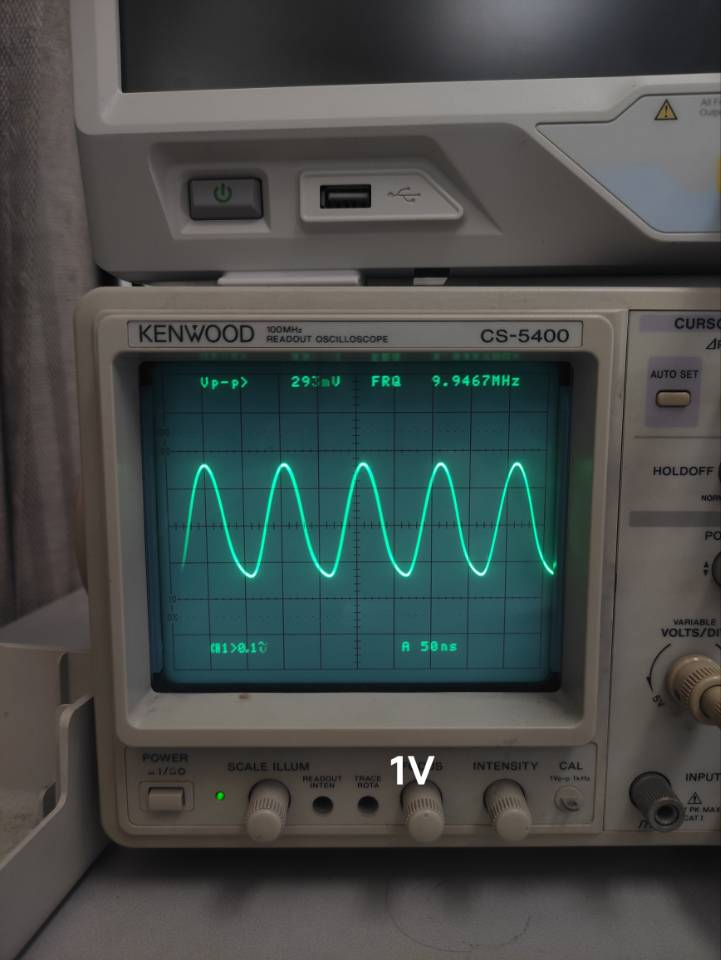
\includegraphics[scale=0.8]{4}
                    \caption{零状态响应2\label{fig:2}}
                \end{minipage}
            \end{figure}
    \subsection{实验结果}
            \begin{enumerate}
                \item 由图像可知,零输入响应由初电压开始,遵照指数规律衰减,最后趋于0。时间常数满足$\tau =RC$。
                \item 由图像可知,零状态响应由初电压开始,遵照指数规律增加,最后趋于稳定值。时间常数满足$\tau =RC$。
            \end{enumerate}
    \subsection{误差分析}
        由于示波器线宽的原因以及示波器游标的精度不高,导致的读书误差。
    \section{讨论、心得}
        通过本次实验,我们对一阶RC电路的瞬态响应过程有了更加深入的理解。通过更换电阻电容,我们可以改变电路的时间常数。
        我们也对示波器的使用有了更加深入的掌握。
    \section{思考题}
        \begin{enumerate}
            \item 零输入响应是指电路没有接入外部电源,而是由内部储能元件引起的响应;零状态响应是指内部储能元件储能为0,由外部给予一个激励之后电路产生的响应。
            \item 接好示波器后,转动示波器的TIME/DIV旋钮,观察图像,使得图像趋于稳定,此时扫描和激励同步。
            \item 时间常数表示过渡反应的时间过程的常数。指该物理量从最大值衰减到最大值的$\frac{1}{e} $所需要的时间。即$u_c(t)$衰减为自身的$\frac{1}{e} $ 倍时需要的时间。其反映了过渡过程的快慢,$\tau $过渡过程时间越长。
        \end{enumerate}
\end{document}
